% ************************************
\section*{Introduction}
% ************************************

\begin{frame}{Motivation}
 
\alert{ \emph{So far:} How to use convex optimization to solve problems in quantum mechanics.}

\vspace{\floatsep}

\begin{tikzpicture}[>=stealth]

\node (Cone) at (0,0) {
\includegraphics[width=8em]{gfx/cone}};
\node (Cat) at (7,0) {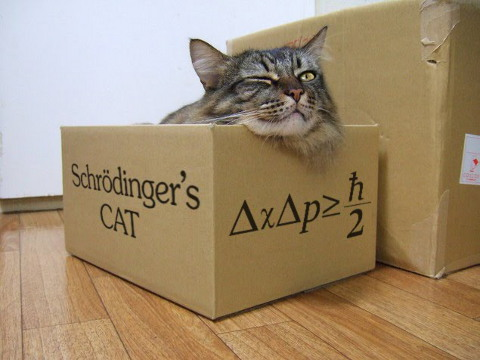
\includegraphics[width=8em]{gfx/cat}};


\draw[->,draw=alerted text.fg, thick] (Cat) to [bend right] node[below,color=alerted text.fg]{!} (Cone);

\visible<2->{\draw[->,draw=structure.fg, thick] (Cone) to [bend right] node[below,color=structure.fg]{?} (Cat) ;}

\end{tikzpicture}

\vspace{\floatsep}

\visible<2->{\structure{\emph{Here:} How to use quantum mechanics to do convex optimization}}

\end{frame}
